% to submit via
% https://www.easychair.org/account/signin.cgi?timeout=1;conf=pyhpc2013
% max 10 pages
\documentclass[conference]{IEEEtran}
%
\usepackage{listings}
\usepackage{url}
\usepackage{todo}
\usepackage{xcolor}
\newcommand\see{\emph{cf.\ }}

\usepackage{tikz}
\usetikzlibrary{positioning}
\usetikzlibrary{shadows}
\usetikzlibrary{arrows}
\usetikzlibrary{shapes}


\lstset{language=python,morekeywords={cimport, cdef, with},
basicstyle=\ttfamily, keywordstyle=\bf, stringstyle=\color{gray},
captionpos=b}

\begin{document}
% update listing numbering
\renewcommand{\thelstlisting}{\arabic{lstlisting}}
%
\title{Compiling Python Modules to Native Parallel Modules Using Pythran and
OpenMP Annotations}

\author{
    \IEEEauthorblockN{Serge Guelton\IEEEauthorrefmark{1}, \IEEEauthorrefmark{2}}
    \IEEEauthorblockN{Pierrick Brunet\IEEEauthorrefmark{2}}
    \IEEEauthorblockN{Mehdi Amini\IEEEauthorrefmark{3}}
    \newline
    \IEEEauthorblockA{\newline\IEEEauthorrefmark{1}
        {\'E}cole Normale Sup{\'e}rieure, D\'{e}partement d'Informatique, Paris,
        France}
    \IEEEauthorblockA{\newline\IEEEauthorrefmark{2}
    T{\'e}l{\'e}com Bretagne, Plouzan{\'e}, France}
    \IEEEauthorblockA{\newline\IEEEauthorrefmark{3}
    SILKAN Inc., Los-Altos, USA}
}

\maketitle

%
\begin{abstract}

    High Performance Computing users traditionally rely on low-level, compiled
    language such as C or FORTRAN to perform compute-intensive tasks. As a
    consequence, it is a common situation to have High Performance Computing
    application written in a high-level language such as Python, calling native
    routines for compute-intensive tasks. To improve development speed and
    reduce maintenance costs, using a higher-level language like Python seems
    attractive. While it is usually associated with low performance, several
    solutions such as Cython, Numba, Parakeet or Pythran offer to automatically
    or semi-automatically turn Python functions into native ones.

    One of the key points required to match the performance of native
    applications is the ability to write parallel applications. This paper
    studies the addition of OpenMP directives, a popular model to describe
    parallelism in C/C++/FORTRAN applications, to Pythran, an automatic compiler
    from a subset of Python to C++. It shows that scientific Python applications
    annotated with OpenMP directives can be turned by an automatic compiler into
    native applications that run within the same order of magnitude than
    manually-written ones.
\end{abstract}

%
\section{Introduction}

Since its birth in December 1989, the Python language~\cite{rossum97} has proved
to be useful in various domains, ranging from system administration to web
services, thanks to its dynamicity, expressiveness, rich ecosystem and
``batteries included'' standard library. It is also widely used in scientific
computing~\cite{Oliphant2007}, thanks to the \texttt{numpy} module and the
SciPy~\cite{scipy} project which provide a set of scientific and numeric tools,
ranging from linear algebra to ordinary differential equation solvers or generic
algorithms.

It is now heading toward High Performance Computing (HPC), either as a glue
language used to bind several native libraries together, or to support whole
applications in Pure Python. However, the prohibitive overhead of the language
implied by its interpreted and highly dynamic nature prevents its usage for the
most performance-critical code sections, where native code is generally used.
The SciPy modules partly overcome this issue through the usage of low-level
routines written in C or Fortran and encapsulated in Python \emph{native}
modules. Moreover, its core data structure, the multi-dimensional
array~\cite{numpyarray2011}, has been designed so that the underlying data are
available to both native modules and the Python interpreter without conversion
cost. Yet when a new function not already part of an existing module is
required, one has to write it in C or FORTRAN.

The hybrid approach, where an application contains a mix of interpreted and
native code, is getting widespread in the Python landscape.
It is also the recommended approach to write applications that make use of fine
grain parallelism, as Python parallelism support is only suitable for
coarse-grain parallelism.
To allow the user to write native functions without having to write the
boilerplate glue code that turns Python object into native structures back and
forth, the SciPy package provides the \texttt{weave} module. It makes it
possible to bundle C code snippets into Python code. They are then compiled and
loaded at runtime. Other project like PyCuda or PyOpenCL offers the same
convenience to target hardware accelerators.

This paper presents the addition of OpenMP, a popular standard to turn
sequential C, C++ and FORTRAN application into parallel applications, to the
Pythran~\cite{pythran2013} compiler, a compiler that turns Python modules into
C++ meta-programs.  Section~\ref{sec:python-parallel} gives an overview of
existing approaches to compile Python functions or modules and shows a critical
lack of parallelism support. It also emphasises on the need for a
backward-compatible approach. Section~\ref{sec:python-static} presents the
Pythran compiler and the underlying runtime library.
Section~\ref{sec:python-openmp} studies the validity of using OpenMP directives
within the Python language in
% I would dispute the fact that OpenMP is "fine-grain", we're not talking about % vectorization here.
order to add fine-grain parallelism support to Python in the context of Pythran.
Finally, the Pythran compiler is benchmarked on several scientific kernels and
compared to Cython, Numba and Parakeet in Section~\ref{sec:validation}.

%=========================================================
\section{Parallel Computations in Python}\label{sec:python-parallel}
%=========================================================

% Mehdi area => era, Serge: validate?
% I also wonder the rational of using parallelism when performance are bad
% because language is bad…
In the many-cores era, it is mandatory to exhibit parallelism to balance the
performance limitations of scripting languages, as described in~\cite{choy05}
in the context of the MATLAB language, or in~\cite{mals07} in the context of
the R language. In the context of Python, most approaches have focused on
fork-based parallelism.

\subsection{Python and Parallelism}

Parallel computations are supported by the Python standard library through the
\texttt{multiprocessing} module. It spawns several interpreters that
communicate through Inter Process Communication (IPC), using Python built-in
object serialization. This approach is only viable for compute-intensive
independent tasks, since the communication and synchronization overheads are
much greater than a light-weight threaded approach.

The standard \texttt{threading} module also makes it possible to start several
light-weight threads within the same interpreter, but this lower-level approach
is not applicable to HPC, because of a specificity of CPython, the \emph{Global
Interpreter Lock}~\cite{gil2012}.\footnote{Other Python interpreters, such as
IronPython or Jython, do not have a GIL.} This lock ensures that only one thread
is active at a time in the interpreter. While it enables the possibility of
cooperative threads, say for a GUI, it does not take advantage of multiple
cores. However, there are two notable exceptions: the GIL is released on I/O,
and the GIL does not prevent the use of threads inside native modules, where the
user has full control.

To illustrate the limitations of these two approaches, we used the CPU-bound
Buffon's needle algorithm to estimate the value of $\pi$. A sequential version
parallelized using the two approaches is illustrated in
Listing~\ref{lst:buffon-python}. When comparing their respective execution time
using 4 cores, it appears that the version that uses the \texttt{threading}
module runs $\times 1.46$ the execution time of the sequential version. GIL
contention actually \emph{increases} the execution time. The version that uses
\texttt{multiprocessing} provides a speedup of 3 over the sequential version
while a speedup of 4 would be expected for this kind of application.

\begin{lstlisting}[float, label={lst:buffon-python}, caption={Implementation of
sequential and parallel version of the Buffon algorithm in Python.}]
def buffon(darts, _ = 0):
  hits = 0
  for i in xrange (0, darts):
    x, y = random(), random()
    dist = sqrt(pow(x, 2) + pow(y, 2))
    if dist <= 1.0:
      hits += 1.0
  # hits / throws = 1/4 Pi
  pi = 4 * (hits / darts)
  return pi

from threading import Thread
from multiprocessing import Queue
def threaded_buffon(d):
  def work(darts, queue):
    queue.put(buffon(darts))
  n = 4
  q = Queue()
  threads = [
    Thread(target=work, args=(d//n, q)),
    Thread(target=work, args=(d//n, q)),
    Thread(target=work, args=(d//n, q)),
    Thread(target=work, args=(d//n, q)),
  ]
  map(Thread.start, threads)
  map(Thread.join, threads)
  return sum(q.get() for _ in threads)/n

import functools
from multiprocessing import Pool
def multi_buffon(darts):
  n = 4
  p = Pool(n)
  return sum(p.map(functools.partial(buffon,darts/n), range(n)))/n
\end{lstlisting}

Another widely used solution is the module \texttt{IPython.parallel}, which supports many
different styles of parallelism including: single program, multiple data (SPMD)
parallelism, multiple program, multiple data (MPMD) parallelism, message passing
using MPI, task farming, and data parallel.
%FIXME: to be continued...

There have also been several approaches to replace the GIL by Transactional
Memories~\cite{Riley2006,Tabba2010} but none of them made its way to the
mainstream interpreters. As a consequence, Python developers need to write
multi-threaded native modules in order to fully benefit from multiple cores.
This leads to a kind of computations referred as \emph{hybrid computations}.


\subsection{Hybrid Computations}

In the context of interpreted languages, \cite{dongara2007} defines a
computation as \emph{hybrid} when part of the code is interpreted, and part of
it is executed natively.

It is now common for scripting language to have C bindings. To take advantage of
compiled code, and to overcome the GIL limitations, Python developers have to
write parallel C/C++ functions and the associated boilerplate based on the
Python C API~\cite{pythoncapi}. Tools have been developed to relieve the user
from this cumbersome task, notably SWIG~\cite{swig2003} that relies on an
interface specification supplied by the programmer to generate the glue, or
\texttt{boost::python}~\cite{boostpython2007} that relies on C++ templates and
type overloading facilities to guide translation.

An opposite approach consists in using the host language ---herein Python--- to
describe both parts of the system, i.e.\ the hybrid and the native. An automated
tool performs the translation to native code of a specific part of the
application, generally the compute-intensive one where parallelism has been
expressed in some ways.
Therefore, developers not familiar with lower level languages or not eager to
invest the additional development time can still benefit from a fair performance
boost.
This approach is the subject of many studies that can be classified according to
their compatibility with the host language.

\subsubsection{Backward-Incompatible Approaches}

A constraining (from the performance point of view) aspect of the Python
language is its type system. It implies that each method call is resolved
dynamically, even a simple add operation. It comes at no surprise that many
approaches restrain the Python language to add a static typing overlay.  Also,
only two types of integers (64-bits integers and multi-precision integers) and
one type of floating point type (double-precision floats) are available in
Python, so using a type with the appropriate size may lead to significant
performance boost.

Cython~\cite{cython2010} is an hybrid Python/C dialect. It extends the Python
syntax with typing information, calls to native functions from third party
libraries, and a limited set of parallelism constructs, such as the possibility
to define parallel loops, but no task parallelism. When possible, it unboxes
Python variables to improve performance. Without type annotations, the
performance improvement is not terrific, but given enough type annotation,
Cython can generates code that runs as fast as its C equivalent, while
maintaining a syntax close to Python.

PLW~\cite{dongara2007} and \texttt{Scipy.weave} both propose another approach
that directly mixes Python with C, using raw strings to hold the C code. PLW
also supports parallel directives that are limited to parallel for loops.
PyCUDA and PyOpenCL~\cite{klockner2012} also target accelerators by mixing
Python with kernels embedded as raw strings containing accelerator code.

The main drawback of these approaches % Reviewer 4 not happy with this
is that they require to modify in a
backward-incompatible way the original code. They require to learn a new
dialect, and the long-term preservation of this investment is not ensured.
Moreover, some of these approaches have no fallback if the code were to be
deployed in an environment where the parallelizing tool/module is not available.
For instance, once a code has been ported to PyCUDA and transformed into CUDA
code embedded in Python strings, there is no way back and the developer has to
maintain two versions of the algorithm.

\subsubsection{Backward-Compatible Approaches}

Most backward-compatible approaches also % Reviewer 4 not happy with this
require to modify the input program.
They do not extend the Python language, but restrict it. As a consequence, they
remain compatible with the original language and do not suffer from the
drawbacks of the previous approaches. They also benefit from existing tools
associated to the language.

Copperhead~\cite{copperhead2011} is a functional, data parallel language
embedded in Python. It uses $n$-uplets, NumPy arrays and lists as its core data
structure and prohibits usage of many control-flow operators such as loops,
enforcing the use of the \texttt{map}, \texttt{filter} or \texttt{reduce}
intrinsics to exhibit parallelism. But it can be efficiently compiled to either
CUDA or C++ with calls to the Thrust\footnote{\emph{cf}.
\texttt{http://thrust.github.com/}} library. Python decorators are used to
identify hot-spots that are JIT-compiled to native code.

The numba~\footnote{\emph{cf}.\ \texttt{https://github.com/numba/numba}}
compiler uses additional type information to generate sequential LLVM bytecode.
Parakeet~\cite{parakeet2012} follows an approach similar to numba, that is
Python to LLVM bytecode translation, but limits its scope to the numpy package,
only supporting a small subset of the Python language. Additionally, it supports
implicit parallelism using an implicit mapping between numpy functions and a set
of parallel primitives including \texttt{map}s \texttt{scan}s and
\texttt{reduce}s. These two approaches use Just-In-Time(JIT) compilation and do
not suffer from backward-incompatibility issues. When meeting an unsupported
construct, numba falls back to Python C-API calls, while parakeet raises an
exception.

Tools such as PyPy~\cite{pypy2009}, a Python interpreter with a tracing JIT, or
Shed~Skin~\cite{shedskin2006}, a Python to C++ compiler are also viable ways to
enhance Python performance. However Shed~Skin does not provide support for
fine-grained parallelism beyond what the standard library proposes. PyPy is
heading toward STM for parallelism support.

To be completely backward compatible, it has to be possible to run the input
code in an environment that is not aware of the existence of the parallelizing
solution. This principle is not respected by parallel libraries, but code
annotations partially satisfy it. This is where parallel annotations shine: the
original code remains mostly compatible with a compiler that is not aware of the
annotations, while taking the annotation into account turns the sequential code
into parallel code.

%FIXME: why not cite OpenMP 4.0 (aka the latest)?
This article proposes to combine OpenMP~\cite{openmp3.1} parallel annotations
with the Python subset supported by the Pythran compiler to make it possible to
write fine-grain parallel applications in Python, while being fully backward
compatible with both the Python language and the sequential algorithm. It
implies that:

\begin{enumerate}

    \item any Pythran code can be run (sequentially), with no module dependency
        or code change, by any Python interpreter;

    \item parallelism is explicit and incrementally added to the original code
        through directives.

\end{enumerate}

%=========================================================
\section{Static Translation of Python Programs}\label{sec:python-static}
%=========================================================

Pythran~\cite{pythran2013} is a subset of Python designed for scientific
computing. It is implicitly statically typed and supports most Python constructs
except those that involve introspection (e.g.\ \texttt{getattr}) or runtime
compilation (e.g.\ \texttt{eval}). A few standard modules are supported in
addition to the core language (e.g.\ \texttt{math}, \texttt{random}). The
\texttt{numpy} module is currently only partially supported. User classes are
not supported. The associated compiler turns Pythran code, possibly annotated
with OpenMP and a few function type annotations, into C++ code.

Figure~\ref{fig:pythran-compiler} summarizes its processing: type inference
helps removing most dynamic behavior, and is combined with a high-level runtime
library ---\texttt{Pythonic++}--- to allow a one-to-one mapping between Python
and C++ constructs. Pythonic++ is a template library, i.e.\ it consists
exclusively of a set of headers. Therefore the generated C++ file is easily
distributable and does not depend on Pythran. One could even preprocess this
C++ file to avoid the need of distributing along the Pythonic++ headers.

The purpose of this section is not to dig into the internals
of the compiler, but rather to focus on the impact of the parallelism layer,
especially on the runtime library.

\begin{figure}

\centering
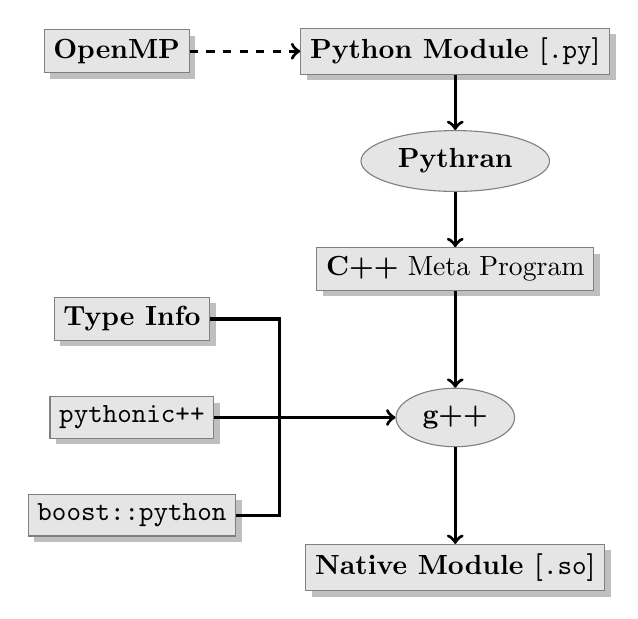
\begin{tikzpicture}[
file/.style={draw=black!50,fill=black!10,rectangle, drop shadow, align=center,
node distance=0.7cm},
    tool/.style={draw=black!50,fill=black!10,ellipse, align=center, node
distance=0.7cm}]
\node[file] (python) {\textbf{Python Module [\texttt{.py}]}};
\node[file] (omp)    [xshift=-2em, left=of python] {\textbf{OpenMP}};
\node[tool] (pythran) [below=of python] {\textbf{Pythran}};
\node[file] (meta-cxx) [below=of pythran] {\textbf{C++} Meta Program};
\node[tool] (gxx) [yshift=-1.5em, below=of meta-cxx] {\textbf{g++}};
\node (empty) [xshift=-1em, left=of gxx] {};
\node[file] (pythonic) [left=of empty] {\textbf{\texttt{pythonic++}}};
\node[file] (annotation)     [above=of pythonic] {\textbf{Type Info}};
\node[file] (boost) [below=of pythonic] {\textbf{\texttt{boost::python}}};
\node[file] (so) [yshift=-1.5em, below=of gxx] {\textbf{Native Module
[\texttt{.so}]}};

\draw[very thick, ->] (python) -- (pythran);
\draw[very thick] (annotation) -| (empty.center);
\draw[very thick,dashed, ->] (omp) -- (python);
\draw[very thick, ->] (pythran) -- (meta-cxx);
\draw[very thick, ->] (meta-cxx) -- (gxx);
\draw[very thick] (boost) -| (empty.center);
\draw[very thick, ->] (pythonic) -- (gxx);
\draw[very thick, ->] (gxx) -- (so);
\end{tikzpicture}

\caption{Pythran compiler workflow.}
\label{fig:pythran-compiler}
\end{figure}

\subsection{Runtime Library Support}

% STL != standard library
Pythran runtime library is based on the C++11 standard library which, unlike its
C++03 counterpart, is thread-safe. It implies that no data dependencies are
added to the original code.

A critical point of the design of the \texttt{pythonic++} runtime library is
memory management, the very same aspect that led to the use of a GIL in CPython.
Memory management is implemented in Shed Skin through the general-purpose Boehm
garbage collector~\cite{boehm1991}, and Cython forbids usage of Python-managed
objects inside parallel regions, thus making memory management explicit for
these parts.

Pythran handles the problem by refusing recursive types, which makes it possible
to solely rely on reference counting for memory management. It can be
implemented through the thread-safe shared pointer mechanism provided by the
C++11 standard library.

Using shared references simplifies memory management, but the counterpart is an
extra atomic operation for each copy.
% UNCLEAR
As it limits parallelism, reducing the number of copies becomes an important
goal.
% end unclear
The move semantic introduced in
C++11 avoids a few copies when working on temporary objects, but argument
passing still implies copies. To avoid a reference increment, one can pass
parameters by reference. Using an inter-procedural memory effect analysis not
presented in the paper, Pythran determines for each argument whether it has to
be passed using reference or const reference to prevent this overhead.

\subsection{Directive Oblivious Translation}

During Python to C++ translation, Pythran adopts a blind strategy: it does not
understand the semantics of the annotations. Instead, it just splits each
annotation into a context-sensitive part ---the variable names--- and a
context-insensitive part ---the clauses---, and attaches them to the proper
construct in the Abstract Syntax tree (AST).

The Pythran compiler ensures a bijective translation between Python constructs
and generated C++ constructs so that the OpenMP directive is regenerated on the
proper construct.
%next sentence unclear
The same approach is used at the expression level, to be
compatible with the \texttt{if} clause.

At the AST level, it means that the Python AST is first reduced to a tree where
all nodes not available in C++ are transformed into a compatible representation.
For instance, list comprehension expressions are turned into function calls or
tuple unpacking is turned in multiple assignments enclosed in a dummy
\texttt{if}. During this transformation
process, an expression is always transformed into a single expression and a
statement is always transformed into a single statement.
Then this AST is converted into a C++ AST meant to be pretty-printed.


\subsection{Transfer Costs}

When passing containers from Python to C back and forth, a copy of the whole
container is made to turn the type agnostic, non-contiguous Python data into
dense typed ones. This extra copy implies an extra cost that is not negligible:
Passing two lists of float from Python to C++ requires as much as half the time
to compute the dot product of the same lists directly in Python. Following
Amdahl's law, this copy overhead greatly hinders the benefits of
parallelization, and is a well known issue.

The traditional solution is to use a native type that exposes a Python interface
and has a constant translation cost. NumPy's \texttt{ndarray} is a typical
implementation of this concept and is the keystone of the Scipy and NumPy
packages. Basically, a NumPy \texttt{ndarray} is a raw C pointer that is exposed
at the Python level. The PEP 3118 defined the API that allows to share
efficiently the embedded data between Python and the native world without
involving any copy. As a tool for scientific computing, Pythran supports such a
structure, implemented as a class wrapping a raw pointer.


%=========================================================
\section{OpenMP Semantical Adaptations}\label{sec:python-openmp}
%=========================================================

OpenMP is a standard API for parallel programming for Fortran, C and C++. It
consists of a set of parallelizing directives and a few runtime library calls.
If OpenMP is not activated, the directives are ignored, thus enabling
incremental parallelization of the original source code while keeping the
original code structure. The languages targeted by OpenMP are statically
compiled. This section studies the semantical adaptation required to use the
same API for a scripting language such as Python.
Listing~\ref{lst:motivating-example} introduces a motivating example through the
computation of $\pi$, featuring a parallel reduction. The C equivalent with
OpenMP directives is given in Listing~\ref{lst:motivating-example-c} for
reference.

\begin{lstlisting}[float, label={lst:motivating-example}, caption={Motivating
example: computing $\pi$ in Python.}]
def pi(nsteps):
  sum, step = 0., 1. / nsteps
  for i in range(nsteps):
      x = (i - 0.5) * step
      sum += 4. / (1. + x**2)
  return step * sum
\end{lstlisting}

\begin{lstlisting}[float, label={lst:motivating-example-c}, caption={Motivating
example: computing $\pi$ in C with OpenMP.}]
double pi(size_t nsteps) {
  double sum = 0., step = 1. / nsteps;
  #pragma omp parallel for reduction(+:sum)
  for(size_t i = 0; i < nsteps ; ++i)
  {
      double x = (i - 0.5) * step;
      sum += 4. / (1. + x * x);
  }
  return step * sum;
}
\end{lstlisting}


\subsection{Directives}

OpenMP directives are held by C/C++ \texttt{\#pragma}, or by Fortran comments.
Most of them apply to structured blocks in C/C++ and delimited by comments in
Fortran. A few directives (e.g.\ \texttt{threadprivate}) are not attached to a
specific instruction.

While Python has a decorator mechanism\footnote{\see PEP 318,
\url{http://www.python.org/dev/peps/pep-0318/} for a more detail explanation of
Python decorators.}, it only applies to functions, methods and classes and does
not allow to attach decorations to other statements.
PLW~\cite{dongara2007}, uses string instructions to hold such decorations. As
Python does not have anonymous block,\footnote{\see PEP340,
    \url{http://www.python.org/dev/peps/pep-0340/} for a discussion concerning
anonymous block support in Python.} one has to create a dummy \texttt{if 1:}
instruction to apply an annotation to a whole block. Pythran uses comments to
hold OpenMP directives, and internally stores them as string instructions.
Alternatively, the syntax \texttt{if 'my annotation':} is also supported.

%what about flush clause which is not linked to a statement?
Many OpenMP annotations are parametrized by clauses that list variables,
specifying their behavior with respect to parallel regions,
e.g.\ \texttt{private}, \texttt{shared}, \texttt{copyin}. They can only refer to
variables that have already been declared. However, there is no variable
declaration in Python, and all variables assigned in a function have the
function scope, called local scope and available through the \texttt{local()}
built-in. As a consequence, all variables that are referenced in a function are
considered when building such variable lists: there is no concept of variable
local to a block. Using the \texttt{default(none)} clause is possible to ensure
no variable gets forgotten when building such lists.

The \texttt{reduction(\emph{operator}: \emph{list})} directive is used to
characterize some data dependencies when performing a parallel reduction. The
list of supported operators depend on the input and backend languages: Python
has \texttt{min}/\texttt{max} operators but C/C++ does not. % C++11 has...
C/C++ have
\texttt{\&\&} or \texttt{||} while Python does not.\footnote{Although similar,
the \texttt{and} and \texttt{or} keywords are not boolean operators in Python.}
The latest OpenMP specifications~\cite{openmp4} describe a way to declare
user-defined reduction but is not implemented in any compiler yet.

The annotated motivating example is given in
Listing~\ref{lst:motivating-example-annotated-v0}. Note that unlike in C,
\texttt{x} has to be listed in a \texttt{private} clause.

\begin{lstlisting}[float, label={lst:motivating-example-annotated-v0},
  caption={Motivating example: computing $\pi$ in Python with OpenMP.}]
def pi(nsteps):
  sum, step = 0., 1. / nsteps
#omp parallel for reduction(+:sum) private(x)
  for i in range(nsteps):
      x = (i - 0.5) * step
      sum += 4. / (1. + x**2)
  return step * sum
\end{lstlisting}

\subsection{Automatic Scoping Computation}

Using function scope for all variables may lead to very long \texttt{private}
clauses. This section describes an algorithm to automatically limit the scope of
a variable declaration so that it can be automatically marked as private, in
a similar manner to C/C++

The whole idea is to compute the minimal nesting depth of a variable usage. To
do so, a \emph{nesting depth} is first associated to each expression. It
lexically corresponds to the indentation level of its instruction, to the
notable exception of the iterator declaration in a for loop, that holds a
nesting depth equals to 1 plus the loop declaration indentation level.

Tracking the nesting depth of all variable use, for instance using def-use % I don't see the need for def-use chains for this! Unless you include some "unaliasing algo"
chains, makes it possible to build a list of nesting depths, one per variable
reference. Computing the min of this list yields the scope of the variable.

For instance, in the motivating example, the \texttt{nsteps} variable is first
defined as argument, then read twice, which gives a def-use chain of
\{DEF, USE, USE\}. The associated nesting depths is
\{0, 1, 1\} so the variable scope is 0. \texttt{i} is defined as a loop iterator
then used in the loop body, which gives a chain of \{DEF, USE\}, with nesting
depths of \{2, 2\} and a scope of 2. Likewise \texttt{x} has a chain of
\{DEF, USE\}, nesting depths of \{2, 2\} and a scope of 2, which means it can be
automatically declared local to the loop, thus not needing to be listed as
\texttt{private}.

To be able to list a variable marked as local, for instance in a
\texttt{lastprivate} clause, the directive accesses are taken into account in
the def-use computations. For instance in
Listing~\ref{lst:motivating-example-annotated-v0}, the chain for \texttt{x} is
\{DEF, DEF, USE\} and the associated nested depths are \{1, 2, 2\} so its scope
is 1 and the variable is not declared local to the loop.

Thanks to this automatic scoping computation, it is possible to write shorter
OpenMP directive, as illustrated in
Listing~\ref{lst:motivating-example-annotated-v1}.

\begin{lstlisting}[float, label={lst:motivating-example-annotated-v1},
  caption={Motivating example: computing $\pi$ in Python with OpenMP and
  automatic scoping.}]
def pi(nsteps):
  sum, step = 0., 1. / nsteps
  #omp parallel for reduction(+:sum)
  for i in range(nsteps):
    x = (i - 0.5) * step
    sum += 4. / (1. + x**2)
  return step * sum
\end{lstlisting}

\subsubsection{Parallel For and Iterators}

The core directive to handle data parallelism is the \texttt{for} directive that
distributes the iteration space of the associated loop among the existing
threads. To be compatible with OpenMP, the loop iteration space has to be
described by a random access iterator with a total order. Integers used as loop
indices in Fortran and C satisfy this conditions, as well as C++ iterators with
the \texttt{random\_access\_tag} trait. But a Python iterator only advances by a
step of one until it is exhausted,
% reviewer 4 disagree with the previous statement
in which case it raises an exception: it
behaves as a forward iterator. To be compatible with OpenMP, these iterators
has to be turned into random access iterators.

The extension of Python iterator to random access iterators is direct for the
standard containers: \texttt{list},\footnote{Python \texttt{list}s behave as C++
\texttt{vector}s.} \texttt{set} or \texttt{dict}. Other iterators require more
care.

Generators, Python objects that behave like iterators, are commonly used in
Python. The simplest one, \texttt{xrange(\emph{start}, \emph{stop},
\emph{step})}, successively yields value starting from \texttt{\emph{start}} to
\texttt{\emph{stop}} by a step of \texttt{\emph{step}}. It is easily extended to
support random access, but it generally does not make sense to use a generator
as a loop iterator, as the relation between two random states of the iterator
may be of an arbitrary complexity.

Generator expressions are generators whose content is built from another
iterator. For instance \texttt{(x*x for x in l)} successively yields the square
of each element in \texttt{l}. They behave like adaptors: they apply a
particular expression on each value of the iterator. It is also the case of the
\texttt{enumerate} builtin, that yields each element of the enumerated iterator
associated with its index. These generators are random access iterators only if
their input iterator is a random iterator itself.

Finally, if the iterator yields a tuple, it is possible to unpack it inside the
\texttt{for} construct, as shown in Listing~\ref{lst:complex-omp-for}. In that
case all the unpacked variables are considered as iterators, especially with
respect to default privatization rules: in the given example, \texttt{i} and
\texttt{v} are private, and the parallel iteration is valid because the input of
\texttt{enumerate} is a list, which allows random access iteration.

\begin{lstlisting}[float, label={lst:complex-omp-for}, caption={Parallel
    loop in Pythran with tuple unpacking.}]
#omp parallel for
for i, v in enumerate([2, 3, 5, 7, 11]):
    print i, ':', v
\end{lstlisting}

Pythran's runtime library is aware of these three kinds of iterators and
supports parallel iteration over random access iterators and iterators adapting
random ones.

\subsection{OpenMP Runtime Library}

OpenMP provides a small runtime library that, for instance, makes it possible to
retrieve the active thread id. All the functions are declared in the
\texttt{<omp.h>} header, and have a default behavior when OpenMP is not
activated.

Providing a binding to these libraries in Python as an \texttt{omp} module does
not raise particular problems, as the signature of these functions only involves
integers, except for the mutex
manipulation. In that case an opaque type is used to represent the native type.

The \texttt{\_OPENMP} macro definition is always provided when OpenMP is
activated, and can be used to detect when OpenMP is not available. Python does
not have a preprocessor, but it is possible to catch the import exception if the
\texttt{omp} module is not found. Listing~\ref{lst:sample-api-usage} showcases
such a call using an example converted from the OpenMP validation suite
presented in next section. The code starts a parallel section using the
\texttt{parallel} directive, spawning several threads. Then each started thread
increases the \texttt{nthreads} variable that has unspecified visibility, thus
is \texttt{shared}. A guard protects the incrementation using the
\texttt{critical} directive. Then one of the thread retrieves the number of
active threads in the parallel region through the \texttt{get\_num\_threads}
function from the \texttt{omp} module. The function should always return
\texttt{True}.

\begin{lstlisting}[float,label={lst:sample-api-usage},caption={Example of
        OpenMP API usage from Python.}]
import omp
def omp_get_num_threads():
  nthreads, nthreads_lib = 0, -1
  #omp parallel
  if 1:
    #omp critical
    nthreads += 1
    #omp single
    nthreads_lib = omp.get_num_threads()
  return nthreads == nthreads_lib
\end{lstlisting}

\subsubsection{Interaction With Pythran Runtime Library}

Pythran already uses OpenMP to parallelize some Python functions. For instance
the \texttt{sum} function from the \texttt{\_\_builtin\_\_} is implemented using
the OpenMP \texttt{reduction} clause. When its first argument proves to be a
\emph{pure} function, it can also call a parallel version of the
\texttt{map} function that internally spawns a parallel region. This leads to a
well known situation with OpenMP, where too many threads may be spawned: nested
parallel regions. OpenMP 4 provides several ways to handle this situation:

\begin{enumerate}

    \item Disabling nested parallelism, through the \texttt{OMP\_NESTED}
        environment variable or the \texttt{omp\_set\_nested} routine.

    \item Setting the maximum number of active levels, through the
        \texttt{OMP\_MAX\_ACTIVE\_LEVELS} environment variable or the
        \texttt{omp\_set\_max\_active\_levels} routine.


    \item Conditionally activating regions or conditionally setting the number
        of threads in a parallel region using the \texttt{omp\_in\_parallel}

\end{enumerate}

The decision is left to the user, depending on its application and OpenMP
implementation.

\subsection{Validation}

A validation suite for OpenMP is proposed in~\cite{wang2012} for C and Fortran.
We ported it to Python, and also extended it to validate the corner cases
specific to Python described in this section. A typical test case is given in
Listing~\ref{lst:openmp-validation}.

\begin{lstlisting}[float,label={lst:openmp-validation},caption={Example of
  Python OpenMP validation test case.}]
def omp_parallel_for_if(loop_count):
  import omp
  using = sum = 0
  #omp parallel for if(using == 1)
  for i in range(loop_count + 1):
    num_threads = omp.get_num_threads()
    sum += i
  known_sum = (loop_count *
              (loop_count + 1)) / 2
  return known_sum == sum and num_threads == 1
\end{lstlisting}

We have used the Pythran tool described in the following % following??
 section to turn each
Python test function into a C++ function with the same directives and runtime
library calls. Apart from the \texttt{threadprivate} directive and the
\texttt{collapse(\emph{n})} clause, all tests were successful.
\texttt{threadprivate} directives were held by global variables not supported in
Pythran yet~; and the C++ code generated by Pythran does not preserve the
perfect loop nesting required by the \texttt{collapse} clause.

%=========================================================
\section{Validation}\label{sec:validation}
%=========================================================

In addition to the experimental validation done using the OpenMP validation
suite presented in Section~\ref{sec:python-openmp}, the performance of parallel
module generated by Pythran from Python module with explicit parallelization
using OpenMP directives has been studied on several situations: first on the
motivating example, then on a synthetic geomatic application. Python and Cython
versions are then compared and finally the effect of OpenMP directives on
Pythran generated code are illustrated in the context of the Python Benchmarks
suite.

The target machine has  8 AMD Opteron 6176 SE cores and 8 GB of RAM. It is
running a Linux kernel 3.10-2-amd64, x86\_64 GNU/Linux. The C++ compiler used is
\texttt{g++} version 4.8.1 and all applications are compiled using the
\texttt{-Ofast} flag. Pythran generated programs are linked with Boost.Python
version 1.54. The Pythran version is extracted from the \texttt{sc2013} branch
of the git repository \url{https://github.com/serge-sans-paille/pythran}. Python
programs are run using the CPython implementation, version 2.7.5. Cython
programs are generated using version 0.19.1. Numba and Parakeet are installed
from the \texttt{master} branch of their respective repositories.
% dommage pour numba et parakeet qui sont les seuls "mal spécifiés"...

\subsection{Motivating Example}

To validate the approach proposed in this paper, let first consider the
motivating example. Figure~\ref{fig:motivating-example-scale} shows how the C
and Python version of the program scale when changing the number of core used.
As a reference, the original Python code runs 41 times slower than the
equivalent C code. As the program is not memory bound and exhibit trivial
parallelism, the C + OpenMP version scales almost linearly. The Pythran + OpenMP
version follows the same pattern.

\begin{figure}

    \caption{Comparison of the scaling of $\pi$ computation function for C and
    Python with OpenMP, depending on the number of active threads.}
    \label{fig:motivating-example-scale}

    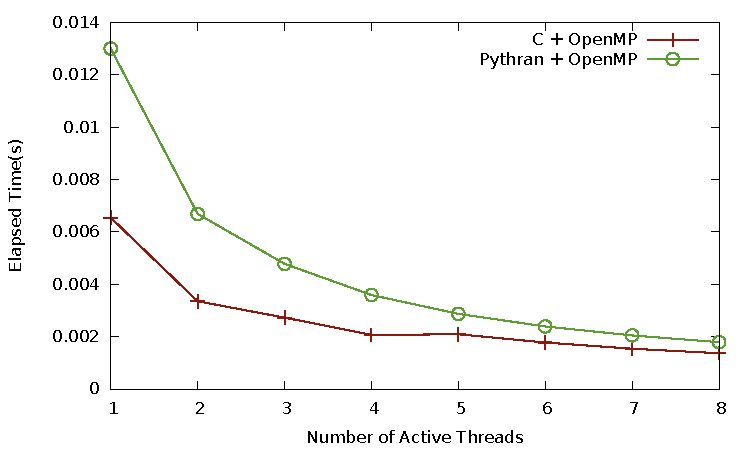
\includegraphics[width=.5\textwidth]{pi_omp_bench.pdf}

\end{figure}


\subsection{Hyantes: a Geomatic Application}

% geomatic or geomatics?? Unify everywhere.
To get closer to a realistic example, we have considered the code of a small
geomatics application, Hyantes. Starting from the C code, we successively
parallelized it using OpenMP, turned it into Python with a Pythran compatible
kernel and parallelized the Python version using the approach described in this
paper. We also measure the number of Source Lines Of Code (SLOC) of the two
versions.  Table~\ref{tbl:hyantes} summarizes the result of this
experimentation. It not only exhibit the use of a high level language
for prototyping, but also shows that it is possible to
turn this prototype into reasonably efficient code through Pythran. It is also
possible to prototype the parallel version while remaining at the Python level.

\begin{table}

    \caption{Comparison of several versions of the Hyantes prototype.}
    \label{tbl:hyantes}

    \centering
    \begin{tabular}{|l|c|}
        \hline
        Language & Source Lines Of Code (SLOC) \\
        \hline
        C       & 102       \\
        Python  & 30        \\
        Pythran & 30        \\
        Pythran+OMP    & 31 \\
        \hline
    \end{tabular}

\end{table}


The Hyantes programs scales relatively well. Figure~\ref{fig:hyantes-speedup}
shows the relative speedup of the application when increasing the number of
OpenMP threads using up to 8 cores.

\begin{figure}

    \caption{Comparison of the scaling of the hyantes application for C and
    Python with OpenMP, depending on the number of active threads.}
    \label{fig:hyantes-speedup}

    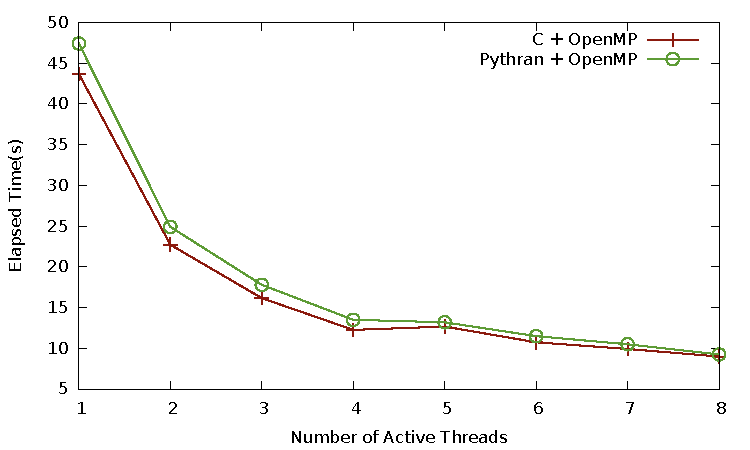
\includegraphics[width=.5\textwidth]{hyantes_omp_bench.pdf}

\end{figure}


\subsection{Comparison with Cython}

We then compare Pythran with Cython. These approaches share some similarities:
they both generate code written in a lower level language, with OpenMP
directives. However, the inputs differ as Cython requires more typing
information than Pythran to generate efficient code, and Cython is not
backward-compatible with Python (outside of \emph{Pure mode}). They translate
explicit fine-grained parallelism through code annotations or specific Python
constructs, respectively.

Pythran exposes the full OpenMP interface to the user, thus enabling both data
and task parallelism, as described in Section~\ref{sec:python-openmp}. It is
not the case in Cython:
%
\begin{itemize}

    \item Only loops can be made parallel, using a new \texttt{prange} generator.

    \item Reductions and variable privacy are inferred, but it chokes on
        reduction on private variables.

    \item The user is responsible from releasing the GIL inside parallel
        regions.

    \item It is impossible to use a function imported from a Python module in a
        parallel region, but it is still possible to use native C functions.

\end{itemize}
%
Listings~\ref{lst:cython-sample} and~\ref{lst:pythran-sample} illustrate the
difference between the two and illustrates the intrusive behavior of Cython.

\begin{figure}

    \begin{lstlisting}[label={lst:cython-sample}, caption={Cython implementation
    of a parallel reduction.}]
from libc.math cimport sqrt
from cython.parallel import parallel, prange
def sum_sqrt(double r):
    cdef int i
    for i in prange(10000000, nogil=True):
        r += sqrt(i)
    return r
    \end{lstlisting}
%
    \begin{lstlisting}[label={lst:pythran-sample}, caption={Pythran
      implementation of a parallel reduction.}]
#pythran export sum_sqrt(float)
import math
def sum_sqrt(r):
    #omp parallel for reduction(+:r)
    for i in xrange(10000000):
        r += math.sqrt(i)
    return r
    \end{lstlisting}
\end{figure}

%Ce n'est pas ce code qui ne donne pas les mêmes résultats avec Cython et Python et Pythran?

The performance of the two approaches is shown in
Figure~\ref{fig:cython-pythran}.  The benchmarked codes are typical
mathematical, image-processing or linear algebra kernels. All these kernels have
been written in Cython and Python ---compatible with Pythran--- and annotated
through the mechanism of each language to exhibit parallelism, then compiled
into native code.  Their execution time when called from the Python interpreter
is measured through the \texttt{timeit} module. All results are normalized
against Cython sequential execution time. They show that while handling code at
a higher level than Cython, Pythran achieves comparable results.
% pythran est bien plus lent quand même :(

The source codes used for these benchmarks are available on the Pythran
repository.\footnote{\see the \texttt{sc2013} branch of the git repository.}

\begin{figure}[ht]
    
\includegraphics[width=.5\textwidth]{cython}
    \caption{Comparison of Cython and Pythran generated code performance.}
    \label{fig:cython-pythran}
\end{figure}


\subsection{Python Benchmarks Test Bed}

The Python Benchmark test bed
(\url{https://github.com/numfocus/python-benchmarks}) is an initiative to
gather relevant numerical python benchmarks and compare several implementations
and compilers. The original benchmarks are slightly adapted to match each
compiler restriction (e.g. lack of support for a particular construct), or
completely rewritten in the target's paradigm (e.g. using PyOpenCL or Theano).
We picked up the targets that did not imply a full rewrite of their input:
Cython, Numba, Pythran and Parakeet, when available and supported.
Additionally, the original Python code is run.

The best execution time out of five run is shown for each code version. If the
code does not compile with a particular compiler, the column is left blank. Two
code versions are shown for Pythran: one compiler without the OpenMP flag set
and one with the OpenMP flag set. The code itself is not modified, only the
compilation flag and the directives. A logarithmic scale is used due to the
generally poor performance of the pure Python version.

%% For the two paragraph below. it is not specified if openmp annotations were
% added by hand. It is misleading since the previous paragraph said
% "The code itself is not modified, only the compilation flag."
Figure~\ref{fig:pb-julia} shows the execution time of the computation of the
julia fractal. It's a highly parallel, compute-intensive code. Pythran and
Cython's version have almost the same execution time, but activating OpenMP
yields an extra $\times 3.95$ speedup when compared to Pythran alone.

\begin{figure}[ht]
    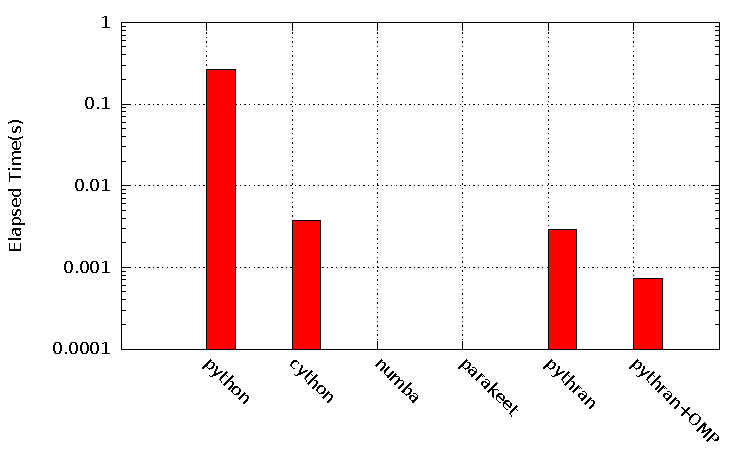
\includegraphics[width=.5\textwidth]{julia}
    \caption{Comparison of Various python Compilers on the Julia benchmark}
    \label{fig:pb-julia}
\end{figure}

Figure~\ref{fig:pb-pairwise} shows the execution time of the computation of a
distance matrix between two random vectors, using a parallel nested loop. On
that example, Pythran slightly outperforms Cython, parakeet and Numba. Taking
into account the OpenMP annotation that flags the outermost loop as parallel
yields an $\times 4.27$ speedup to Pythran.

\begin{figure}[ht]
    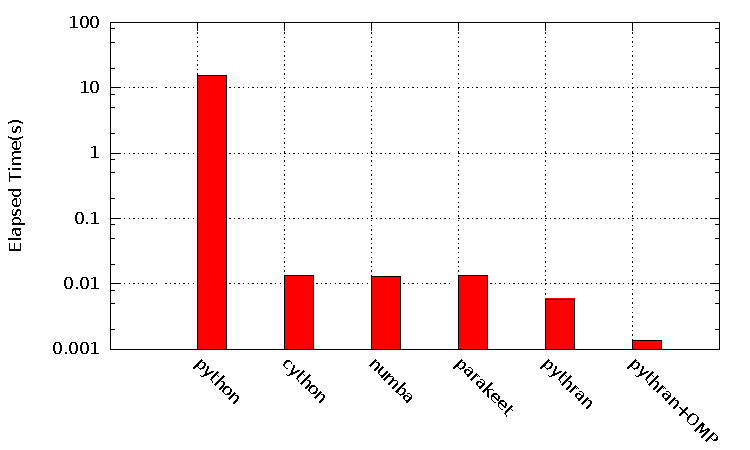
\includegraphics[width=.5\textwidth]{pairwise}
    \caption{Comparison of Various python Compilers on the pairwise benchmark}
    \label{fig:pb-pairwise}
\end{figure}

Figure~\ref{fig:pb-rosen} shows the execution time of the computation of the
third derivative of the Rosenbrock function for a random array input, using
Numpy's vector operations. There is no explicit parallelism in this function but
the vector operation is implicitly parallel. On this example, Cython is on par
with Pythran and slightly faster than Parakeet, but turning OpenMP on makes the
Pythran version run $\times 1.78$ faster than sequential Pythran.

\begin{figure}[ht]
    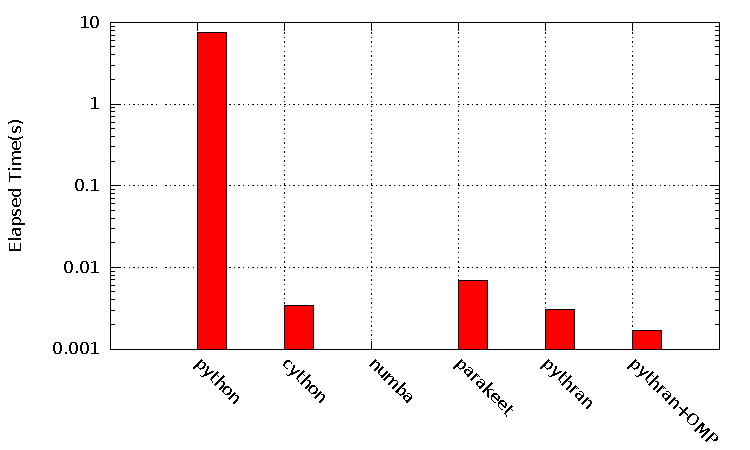
\includegraphics[width=.5\textwidth]{rosen_der}
    \caption{Comparison of Various python Compilers on the rosen\_der benchmark}
    \label{fig:pb-rosen}
\end{figure}

Figure~\ref{fig:pb-growcut} shows the execution time of the computation of one
step of the GrowCut algorithm used in image processing. On this example,
Parakeet performs better than Cython and Pythran and way better than Numba, but
parallelizing the outermost loop with OpenMP gives a $\times 2.65$ speedup to
Pythran that helps it outperform Parakeet.

\begin{figure}[ht]
    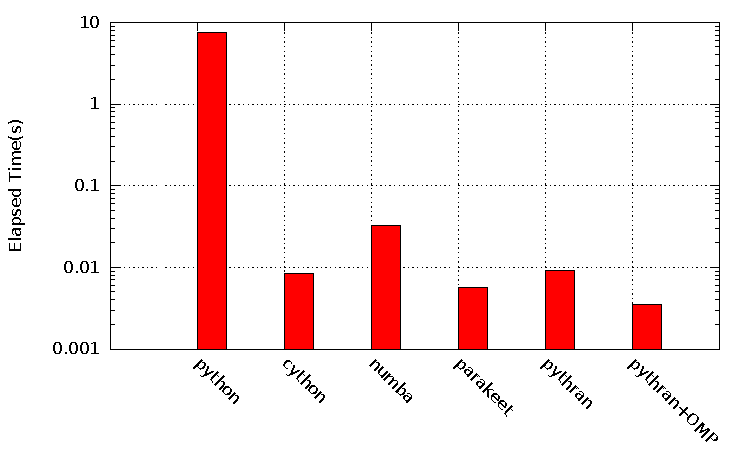
\includegraphics[width=.5\textwidth]{growcut}
    \caption{Comparison of Various python Compilers on the Growcut benchmark}
    \label{fig:pb-growcut}
\end{figure}

It appears that all Python compilers manage to yield significant speedups over
the Python interpreter, each compiler managing some cases better than others.
All the benchmarks exhibit some level of parallelism that are easy to capture
using OpenMP without changing the original algorithm and while maintaining
backward compatibility with the Python interpreter. Some even have a degree of
implicit parallelism that makes parallelization fully transparent to the user.
Taking advantage of this parallelism appears to be the key to reach an
additional performance level.


%=========================================================
\section{Conclusion and Future Work}
%=========================================================

This paper studies the addition of OpenMP annotations to Pythran. It shows that
providing minor semantic adaptations, these annotations enable Python code
to benefit from multi-cores while retaining backward compatibility and without
worrying about the Global Interpreter Lock.

To achieve this goal, we designed Pythran, a translator from a subset of the
Python language to C++. Pythran turns regular Python modules annotated with
OpenMP directives and a few type annotations into native parallel module. The
input module remains compatible with the standard interpreter and the underlying
runtime library is compatible with parallel constructs. While Pythran accepts a
limited input, we extend it progressively and with a great care on its
stability. As such, even if its development is community-based, it is more than
a research prototype and should be usable on real world code.

The approach is compared with Cython, an extension of the Python language used
to generate native module with an hybrid Python-C syntax that also provides
means to exhibit fine grained parallelism. It shows that retaining Python
compatibility does not prevent the achievement of comparable performances.
Comparisons to Numba and Parakeet shows the benefit of using parallelism on the
benchmarks from the Python Benchmark project.

Future work will focus on the extension of the approach to OpenMP 4 and the
\texttt{target} clause that should allow to target accelerator like Intel MIC
from Python.
The \texttt{simd} clause also brings interesting vectorization capabilities that
could be exposed at the python level. There are also several implicit
vectorization opportunities in Python, especially in the list comprehension
construction, that need to be explored.

%=========================================================
\section*{Acknowledgment}
%=========================================================

This work has received fundings from \textsc{silkan} and the French ANR through
the CARP project. The authors thank Adrien \textsc{Merlini} and Alan
\textsc{Raynaud} for their work on the runtime library, Albert \textsc{Cohen},
B{\'e}atrice \textsc{Creusillet}, Fabien \textsc{Dagnat}, Fran{\,c}ois
\textsc{Irigoin} and Ronan \textsc{Keryell} for their valuable reviews.

\bibliographystyle{IEEEtranS}
\bibliography{biblio}


% FIXME reviewer 4
% Fig 2, 3, etc: Please use a different color scheme, or add plot markers to
% the plots for the colorblind among us who can't distinguish thin green and
% red lines from each other.

% FIXME reviewer 4
% Fig 2, 3: I believe a log-log plot or a plot of the overall speedup versus
% number of active threads would be a better way to display the data.

% Remaining reviewer's comments:
% - Is it the intent of the Pythran authors to expose the entirety of the
%   OpenMP API, or just a subset?  Task parallelism?
% - V.C: "Cython is not backwards compatible with Python".  This is false:
%   Cython's Pure Python mode is fully backwards compatible.
% - Figs 5,6,7,8: to do apples-to-apples, what about Cython + prange?
% - Perhaps the only complain is that I would have liked to see the timing for
%   compilation to be included in the article.  Pythran and Cython are very
%   different beasts than Numba or Parakeet in this sense, and the later maybe
%   more useful to compile code that still not exists at compilation time (like
%   user queries, for example).

\end{document}
% vim:spell spelllang=en
% vim:tw=80
